\section{Kronisk obstruktiv lungesygdom}
Kronisk obstruktiv lungesygdom (KOL) er en kronisk inflammatorisk proces, der resulterer i gradvist nedsat lungefunktion. Den kroniske inflammation opstår i luftvejene og lungevævet, hvilket forårsager, at bronkiernes vægge ødelægges og/eller luftvejene forsnævres.\cite{Basisbogen2016}. KOL er beslægtet med to patologier, herunder kronisk bronkitis og emfysem. KOL-patienter oplever ofte begge patologier, men omfanget af disse kan variere fra patient til patient.\cite{Basisbogen2016,Healthguidances2016}

Kronisk bronkitis er luftvejsinflammation med øget slimproduktion og bakteriel infektion. Bronkierne i slimhinden er beskadiget, hvilket medfører en øget slimproduktion. Derudover er antallet af cillia mindsket, hvormed transport af slim og støvpartikler fra bronkierne til svælget begrænses, hvorfor der opstår bakterielle infektioner. Yderligere er slimhinden fortrykket, hvilket medvirker til forsnævring af små og store bronkier. \cite{Frausing2011, Britannica2016}. 

%\begin{figure} [H]
%\centering
%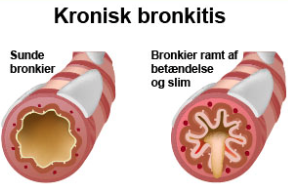
\includegraphics[width=0.5\textwidth]{figures/kroniskbronkitis}
%\caption{Til venstre ses en sund bronkie, mens der til højre ses en bronkie, der er ramt af betændelse og slim. \fxnote{BILLEDE SKAL REDIGERES, KILDEN ER IKKE SÅ GOD, MEN DET BEDSTE BILLEDE JEG KUNNE FINDE} [9]}
%\label{fig:kroniskbronkitis}
%\end{figure} 
\noindent
Symptomerne er langvarig irritation af luftvejene med vedvarende hoste og slimproduktion. Patienter med overvejende kronisk bronkitis betegnes blue bloater. Disse patienterne har ofte lungeinfektioner, cor pulmonale og har type 2 respirationssvigt. Cor pulmonale betegner en trykbelastet og med tiden udvidet hypertrofisk og dårlig fungerende højre ventrikel. Respirationssvigt af Type 2 betyder et lavt iltniveau og højt indhold af kuldioxid. Den dårlige ilttilførsel til ekskrementer og huden samt læber vil medvirke til at disse bliver blålig, hvorfor disse patienter omtales blue bloater. \cite{Healthguidances2016}

Emfysem karakteriseres ved lunge destruktion, dannelse af lungeblærer, tab af elastisk tilbagetrækning og hyperinflation. Emfysem skyldes, at lungernes volumen er øget grundet beskadiget lungevæv, herunder destruktion af elastiske fibre og nedbrydning af væggene i de små lungeblærer. Dette medfører til at overfladen, som lungen har til rådighed ved luftudvekslingen med blodet mindskes, hvorved små bronkier kan klappe sammen og derved lukke under ventilation.\cite{Frausing2011a,Flaschen-Hansen2008}

%\begin{figure} [H]
%\centering
%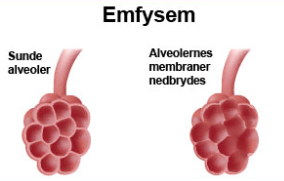
\includegraphics[width=0.5\textwidth]{figures/emfysem}
%\caption{Til venstre ses en sund alveole, mens der til højre ses en alveole, hvor membranen er nedbrudt. \fxnote{BILLEDE SKAL REDIGERES, KILDEN ER IKKE SÅ GOD, MEN DET BEDSTE BILLEDE JEG KUNNE FINDE} [9]}
%\label{fig:emfysem}
%\end{figure} 
 
\noindent
Symptomerne er forpustethed ved let aktivitet, lidt hoste og slim, som kan udvikle sig til anstrengt vejrtrækning og lufthunger ved let aktivitet. Patienter med overvejende emfysem betegnes ofte pink puffer. Disse patienter har ofte kakeksi, tøndeformet brystkasse og har type 1 respirationssvigt. Kakeksi er betegnelsen for alvorlig afmagring eller vægttab med tydelige tegn på nedbrydning af muskelmasse og fedtvæv. Type 1 respirationssvigt er ved lavt iltniveau og normal indhold af kuldioxid. Ved vejrtrækning vil patienternes kroppe blive pustet op og huden vil blive rødlig, hvorfor disse patienter omtales pink puffer.\cite{Healthguidances2016}

Definitionen af KOL beskrives ved ratioen mellem forceret eksspiratorisk volumen i et sekund (FEV1) og forceret vitalkapacitet (FVC). FEV1 måles ud fra, hvad der udåndes i det første sekund efter en maksimal indånding. FVC er udtryk for, hvad der udåndes efter en maksimal indånding målt i liter. Ved tilfælde af KOL er FEV1/FVC under 70 \% af den forventede lungekapacitet. \cite{Basisbogen2016}

Der er flere disponerende faktorer til KOL heriblandt skadelige partikler samt gasser, miljøpåvirkninger og genetiske faktorer. Den hyppigste årsag til KOL er rygning, som fremskynder tab af lungefunktion.\cite{Basisbogen2016,Martinez2016,dsam2016} Foruden rygning kan miljøpåvirkninger have betydning for udviklingen af KOL. Opvækst i et dårligt miljø vil kunne påvirke barnets lunger til ikke at udvikle sig som de skal, hvilket kan resultere i en lavere FEV1. Dertil vil et dårligt arbejdsmiljø kunne medvirke til en accelererende reduktion i FEV1, der ligeledes kan øge risikoen for KOL. \cite{Martinez2016} Dette vil betyde, at en lav eller en accelererende reduktion af FEV1 vil FEV1/FVC-ratioen mindskes. 

KOL udvikles over mange år, dog vil patienten ikke bemærke sygdommen førend lungefunktionen er markant nedsat. Dette betyder, at KOL og dens symptomer som regel først kommer til udtryk efter 50 års-alderen\cite{Lange2015}. Dette kan betyde, at patienter først opsøger en læge, når deres lungefunktion er halveret \cite{dsam2016}. 



